\documentclass{beamer}

\usepackage{hyperref}
\usepackage{epstopdf} 
\usepackage{graphicx}
\usepackage{amssymb}

\title{Central Trigger Board}
\author{ Update \\ Jonathon Sensenig}
\institute{University of Pennsylvania}
\date{}

% position the logo
%\addtobeamertemplate{frametitle}{}{%
%	\begin{textblock*}{100mm}(\textwidth,-1cm)
%		
\includegraphics[height=1cm,width=1cm,keepaspectratio]{figs/Penn-Shield.png}
%\end{textblock*}}

%Add page number to the foot bar
\expandafter\def\expandafter\insertshorttitle\expandafter{%
	\insertshorttitle\hfill%
	\insertframenumber\,/\,\inserttotalframenumber}

%Use an image as the background
%\usebackgroundtemplate{
%	
\includegraphics[width=\paperwidth,height=\paperheight]{figs/bblue3.pdf}
%

%Add logos to title page only
%\titlegraphic{
\includegraphics[width=1.75cm]{figs/DUNElogo_color.png}\hspace*{2.75cm}~
%	\includegraphics[width=3cm]{figs/shield-logotype-whitebkgd-RGB-4k.png}
%}

\usetheme{Copenhagen}
\setbeamertemplate{navigation symbols}{} %NO nav buttons!

% Color modification
\definecolor{MyBackground}{RGB}{255, 255, 255}
\definecolor{jgrey}{RGB}{121, 147, 179}
\definecolor{jred}{RGB}{181,0,0}
\setbeamercolor{background canvas}{bg=MyBackground}
\setbeamercolor{structure}{fg=jgrey}% to modify  immediately all palettes
\setbeamercolor{title}{fg=black}
\setbeamercolor{title in head/foot}{fg=jred}
\setbeamercolor{author}{bg=black,fg=white}
\setbeamercolor{frametitle}{fg=black}

\begin{document}
	\frame {
		\titlepage
		\hspace{0.2cm}
		
\includegraphics[width=10cm,height=2.25cm]{figs/dune_penn_logo.png}
		
	}	
	
	\frame {
	    \frametitle{Modified PTB  1/2}
	    \framesubtitle{}
	    \begin{figure}
	    	\centering
	    		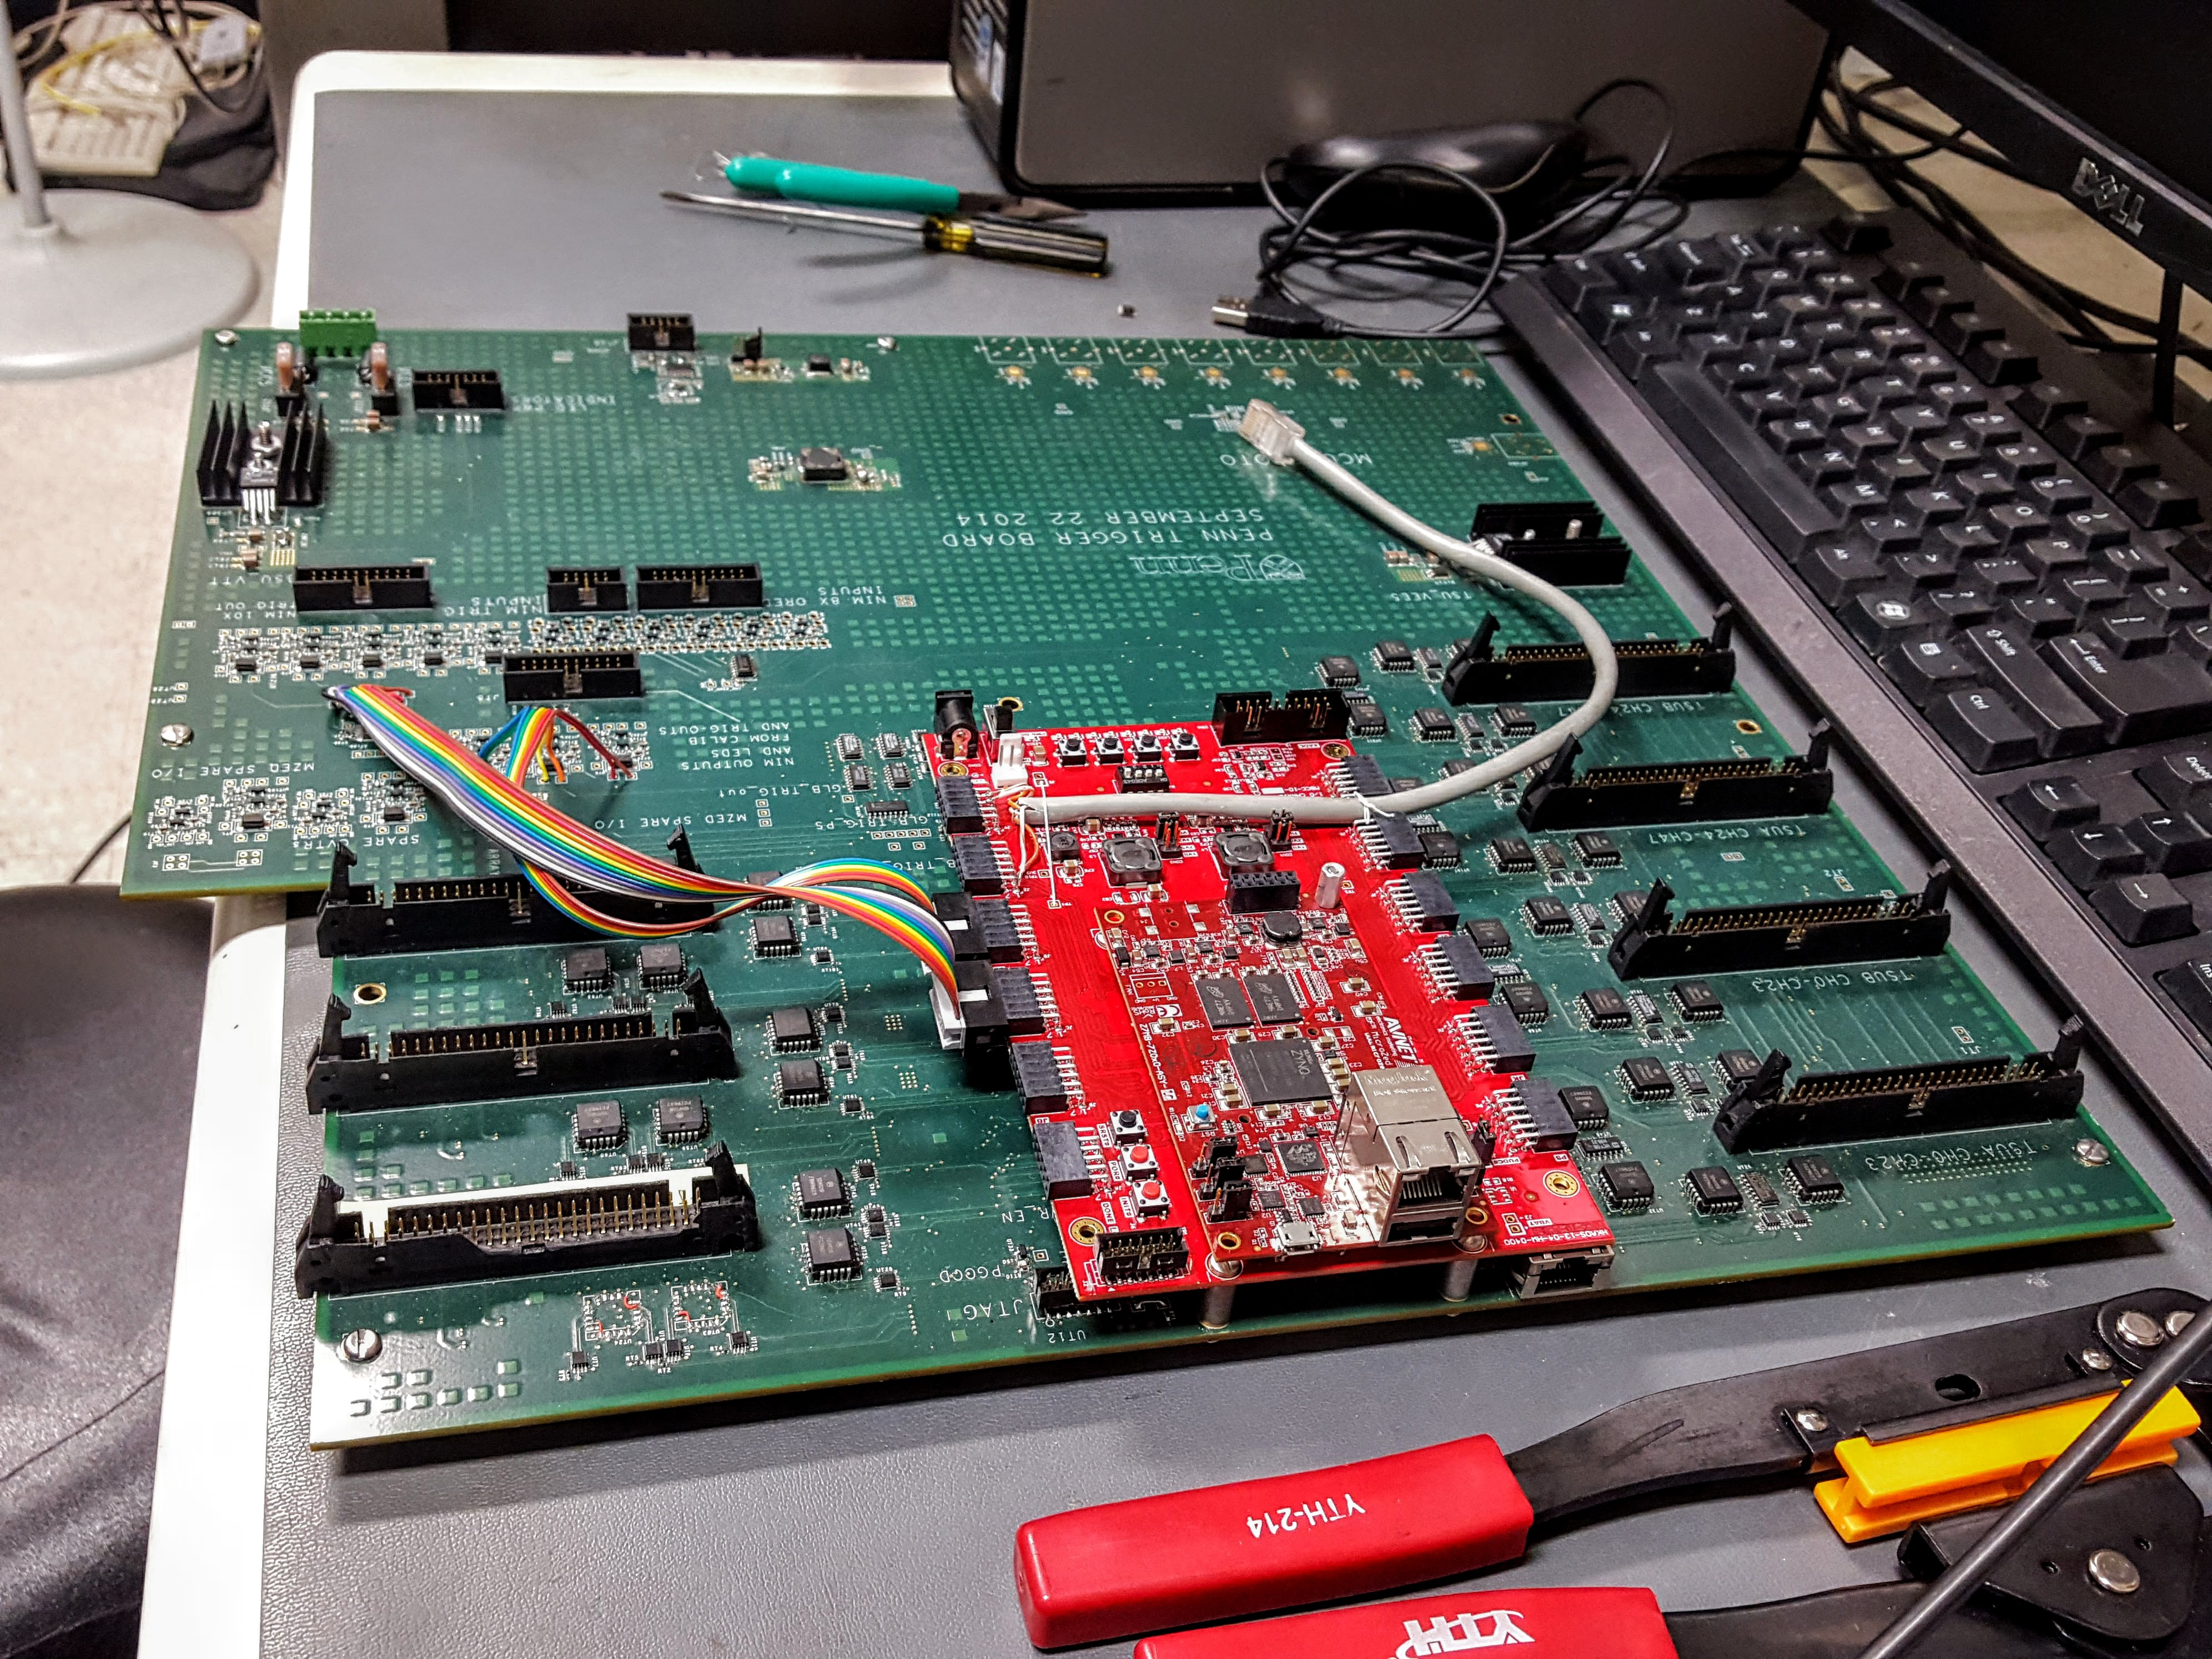
\includegraphics[width=9cm,height=6cm]{figs/ptb_mz.jpg}
	    \end{figure}	
	}
	\frame {
	    \frametitle{Modified PTB  2/2}
	    \framesubtitle{}
		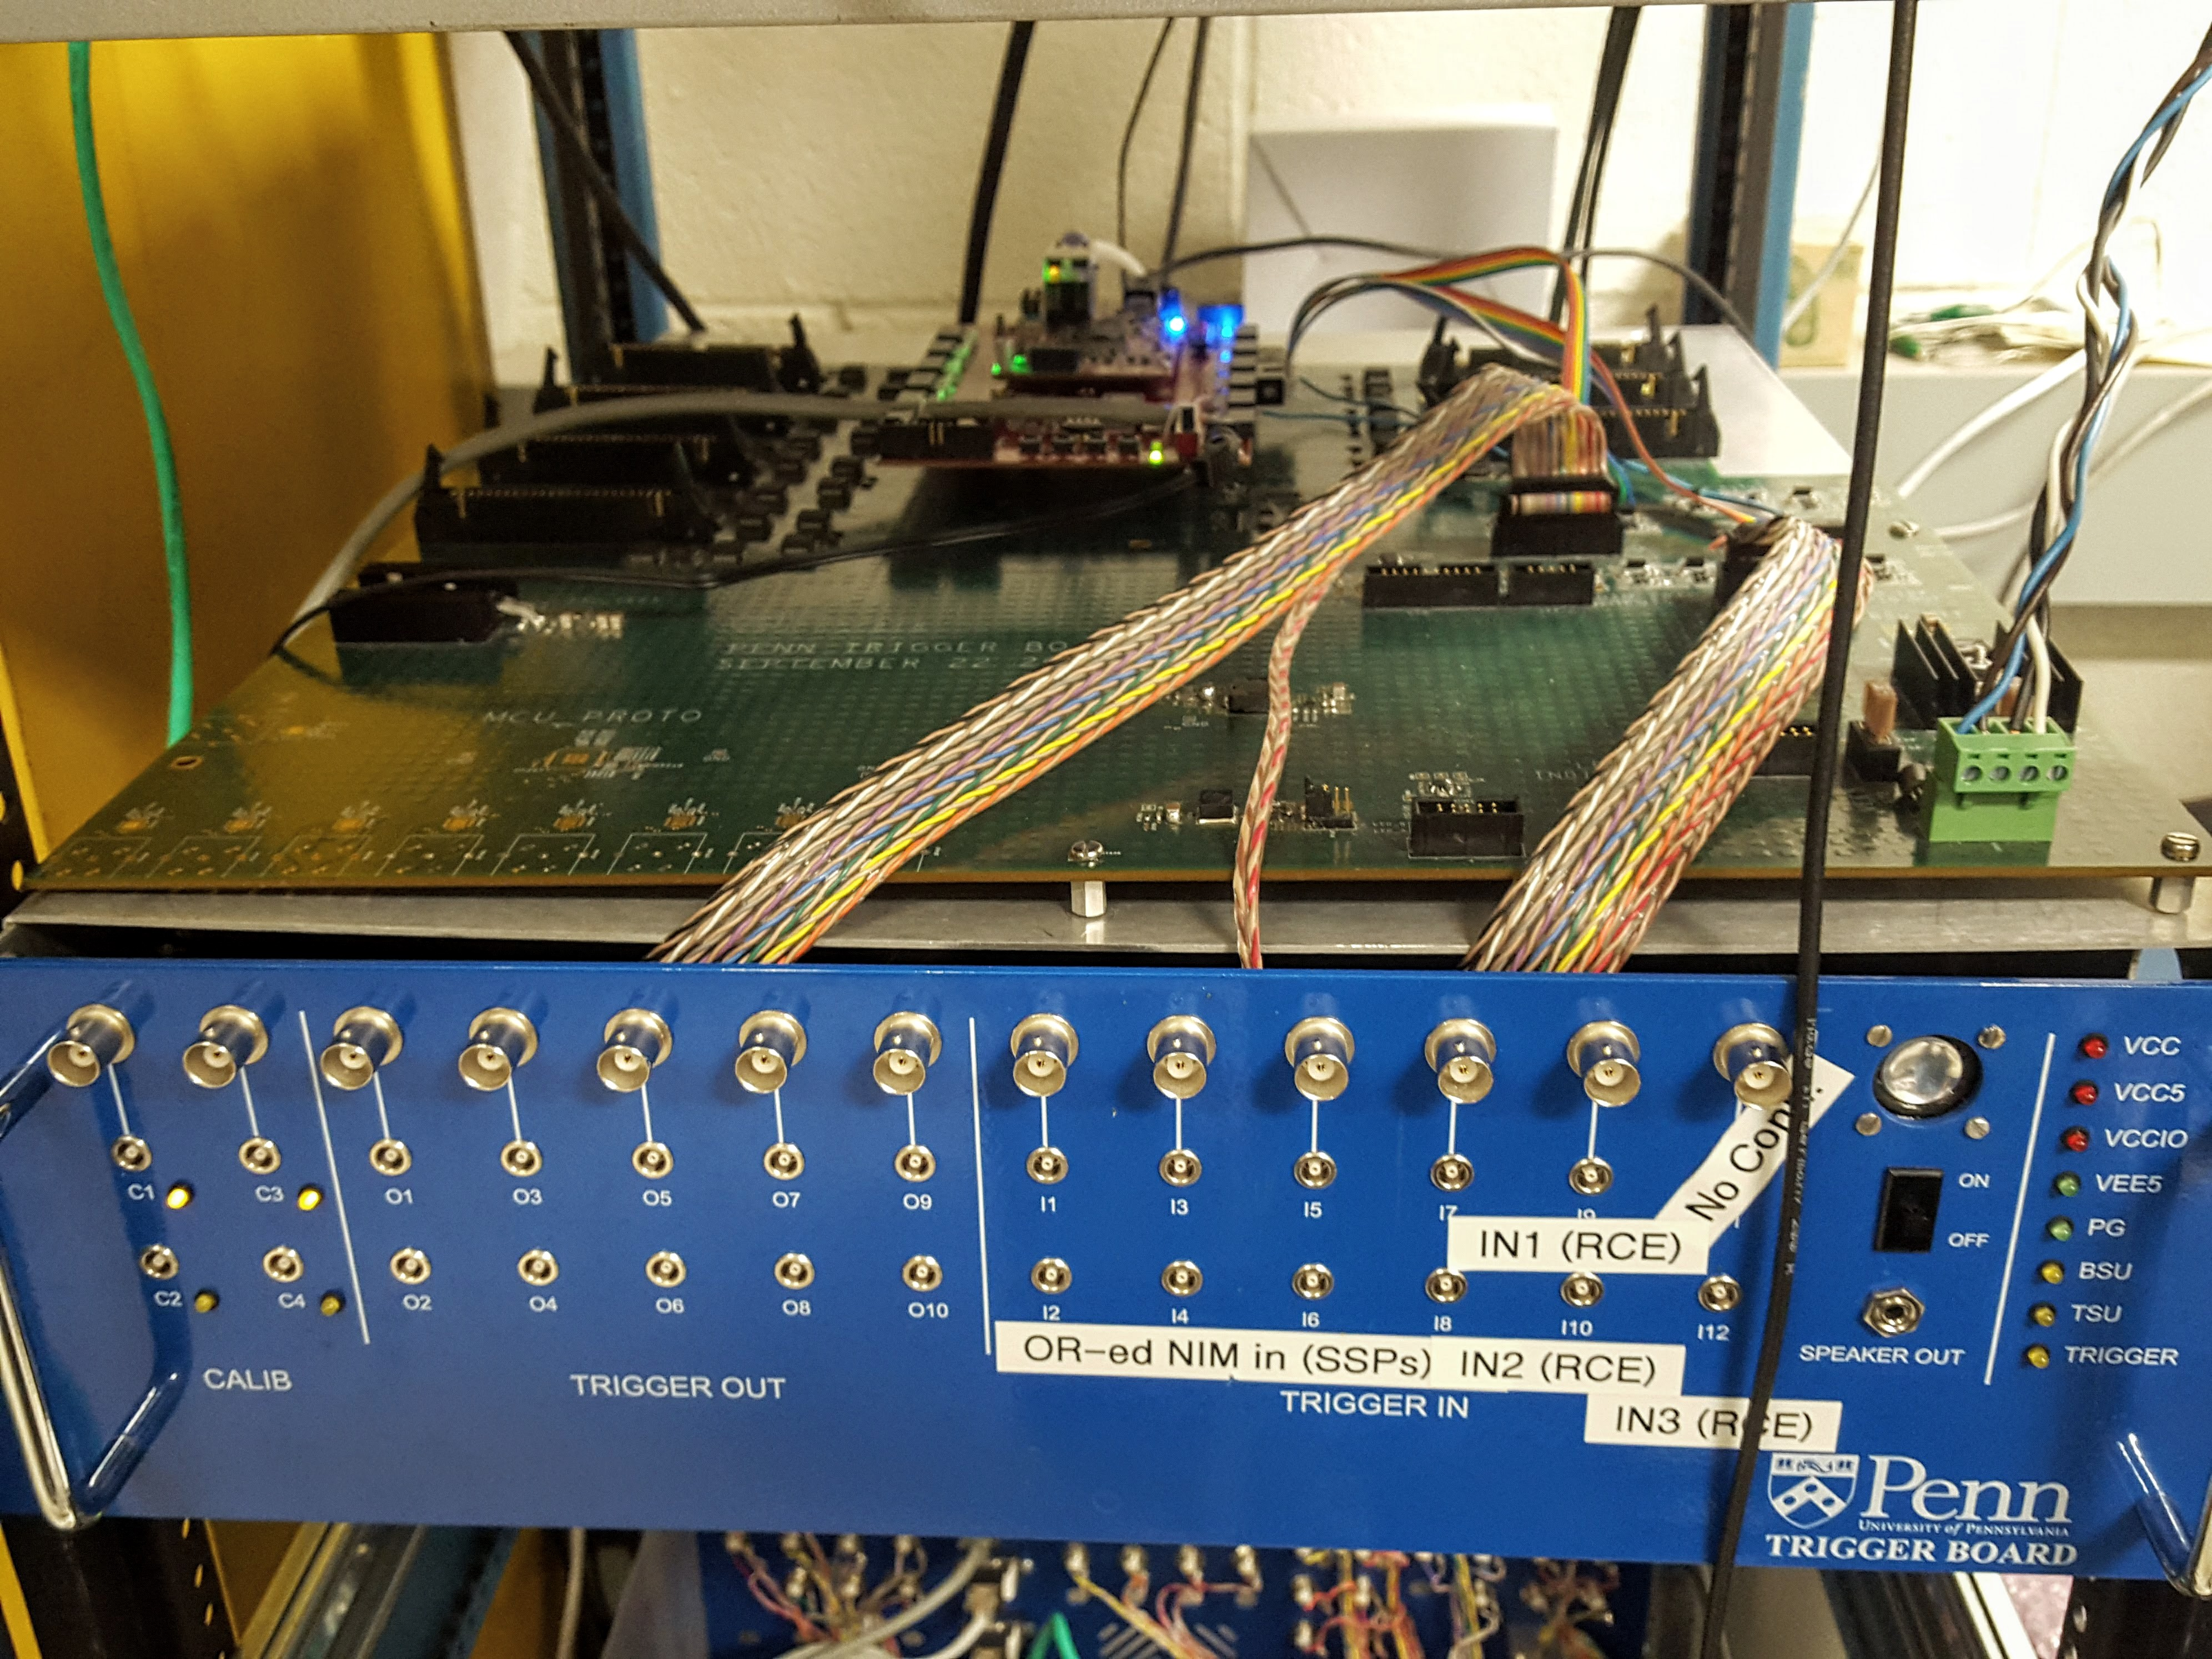
\includegraphics[width=9cm,height=6cm]{figs/ptb_mz_case.jpg}
	}

	\frame {
	\frametitle{Beam Trigger  1/4}
	\framesubtitle{The Beamline as Represented in simulation}
	\begin{figure}
		\centering
		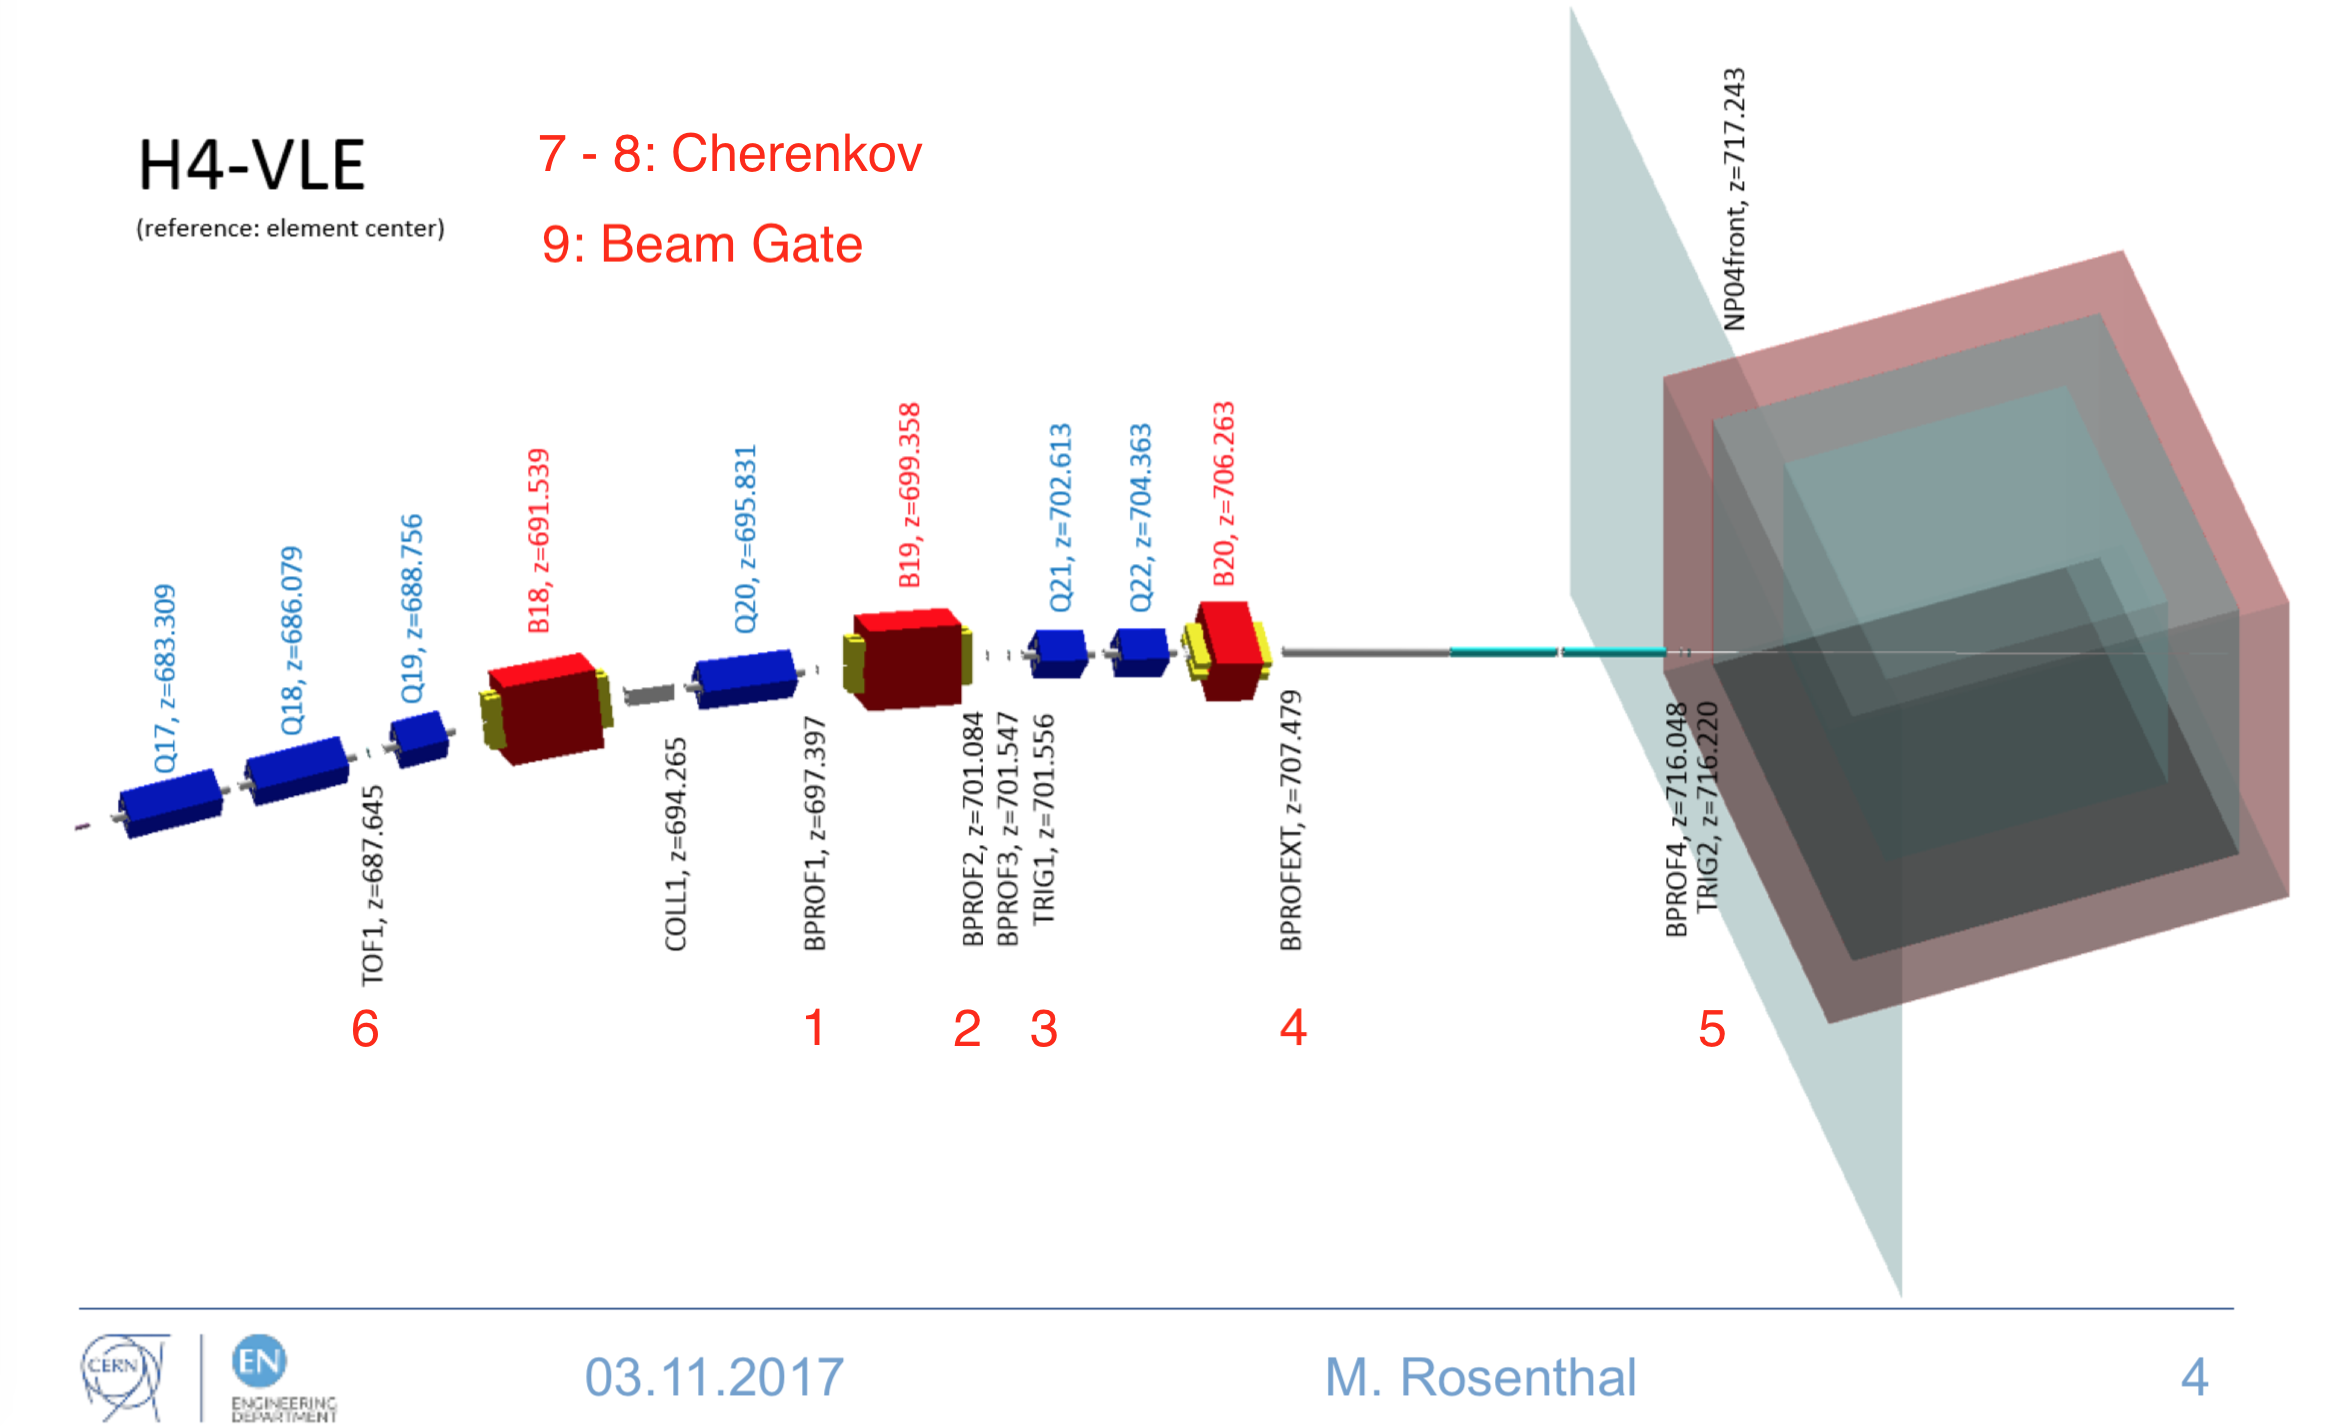
\includegraphics[width=9cm,height=6cm]{figs/h4beam.png}
	\end{figure}
	}

	\frame {
	\frametitle{Beam Trigger  2/4}
	\framesubtitle{Some Questions}
	\begin{itemize}
		\item Is there any reason to trigger if not all fiber trackers fire? Maybe something like $>$3 trackers, low probability of a false trigger and will offset the approx. 6.5\% inefficiency of the trackers.
		\item
	\end{itemize}
	}

	\frame {
	\frametitle{Beam Trigger  3/4}
	\framesubtitle{Jon Paley's Presentation at Collab. Meeting}
	\begin{figure}
		\centering
			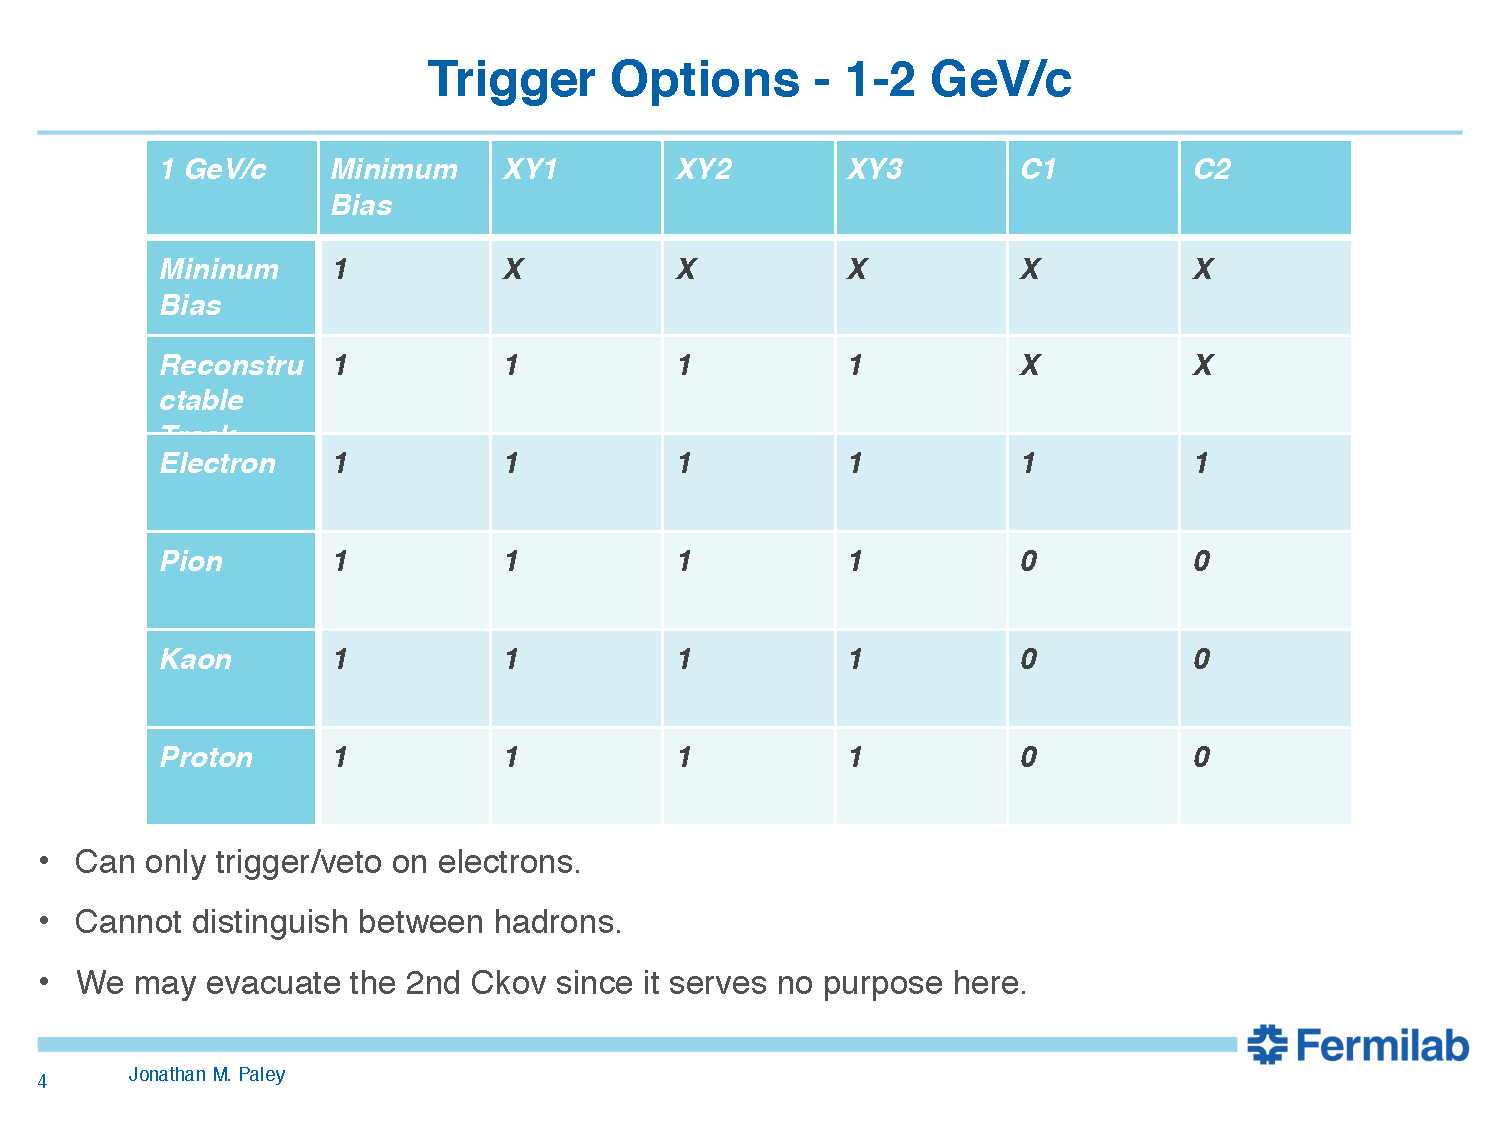
\includegraphics[width=9cm,height=6cm]{figs/2018-01-31_Trigger_Discussion_BI.pdf}
	\end{figure}
	}

	\frame {
	\frametitle{Beam Trigger  4/4}
	\framesubtitle{Beam Triggers Summary}
	\begin{itemize}
		\item Start with all fiber trackers.
		\item Start with 1 - 2 GeV/c triggers since the first run (engineering run) will be with 2GeV/c beam.
	\end{itemize}

	\begin{center}
		\begin{table}[ht]	
			\caption{1-2 GeV/c beam triggers inclusive trigger masks.}
			\centering 
			\begin{tabular}{c c }
				\hline \hline         
				Trigger & $\lbrack$ 8 : 0 $\rbrack$ = $\lbrack$ BG, C2, C1, TOF, BP1-5 $\rbrack$    \\ [0.5ex] 
				\hline 
				No Beam & 0 XX X XXXXX  \\	
				e$^-$ & 1 11 1 11111  \\
				$\pi$/K/p & 1 00 1 11111  \\
				\hline	
			\end{tabular}
			\label{table:bi_trig}	
		\end{table}	
	\end{center}
	}
	
	\frame {
	\frametitle{CRT Trigger  1/}
	\framesubtitle{Channel Mapping of CRT Modules  (ref. Camillo M.)}
	\begin{figure}
		%\centering
		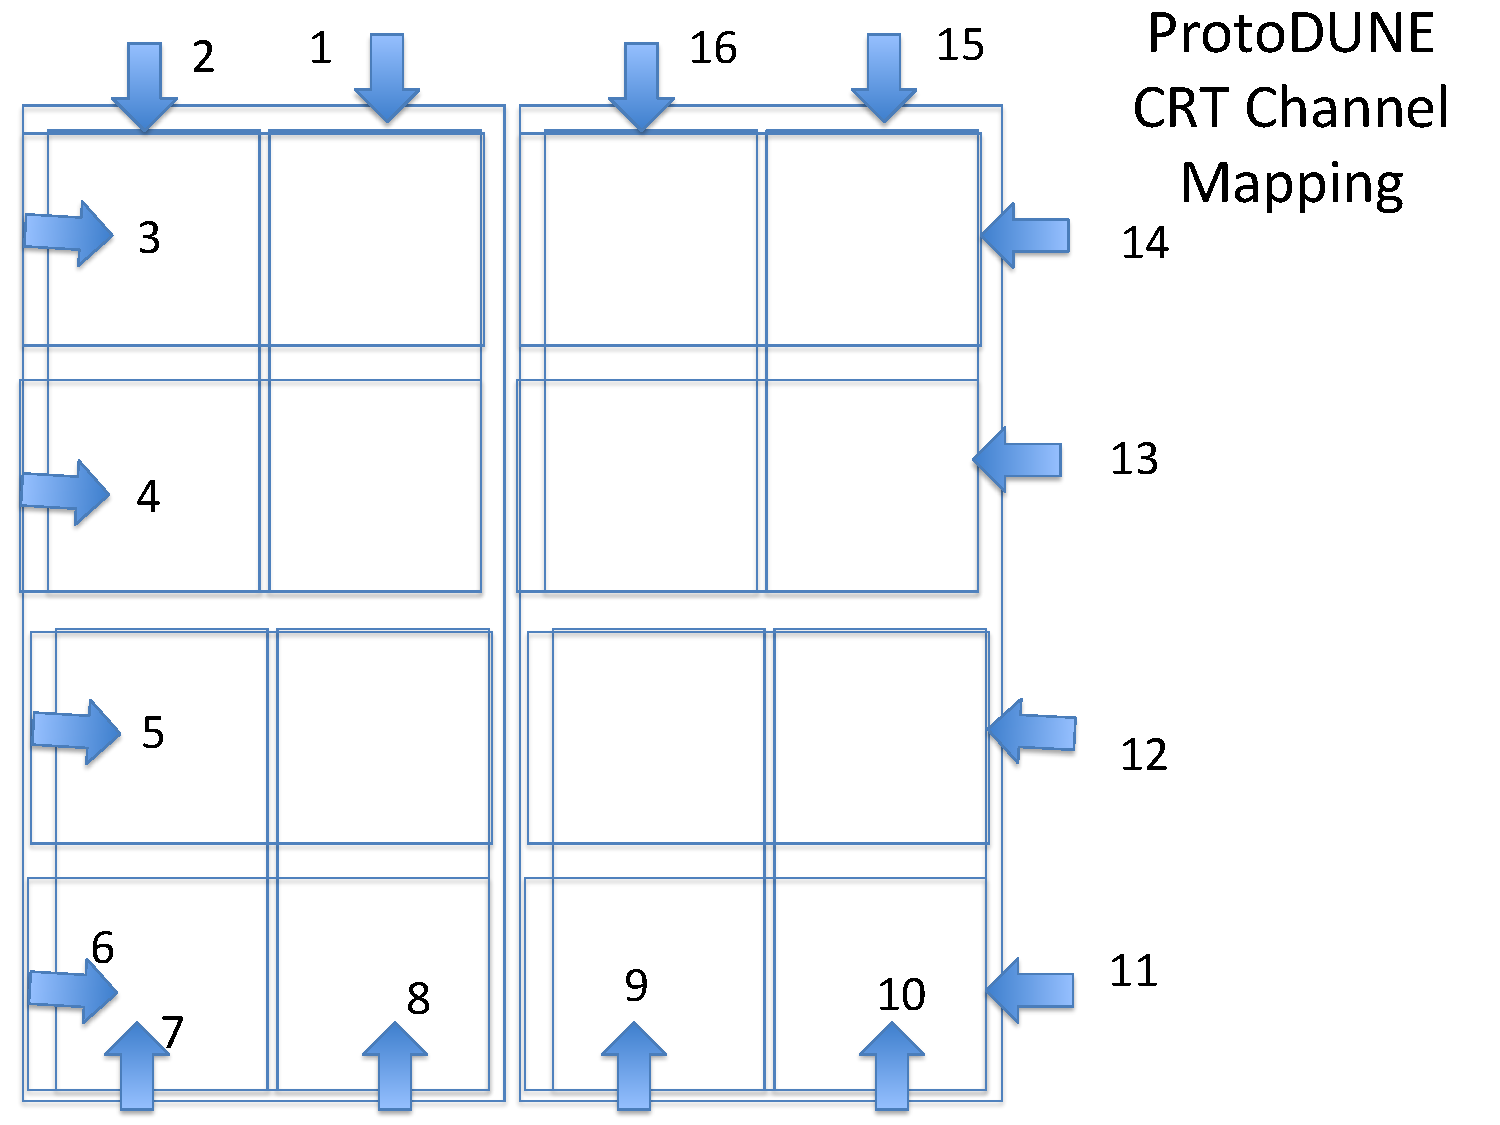
\includegraphics[width=9cm,height=6cm]{figs/crt_mapping.pdf}
	\end{figure}
	
	\begin{itemize}
		\item Front: Channels 1 - 16 $\rightarrow$ Bits [15:0]
		\item Rear: Channels 15 - 32 $\rightarrow$ Bits [31:16]
	\end{itemize}
}

	\frame {
		\frametitle{CRT Trigger  1/}
		\framesubtitle{CRT Triggers Top View}
		\begin{figure}
			\centering
			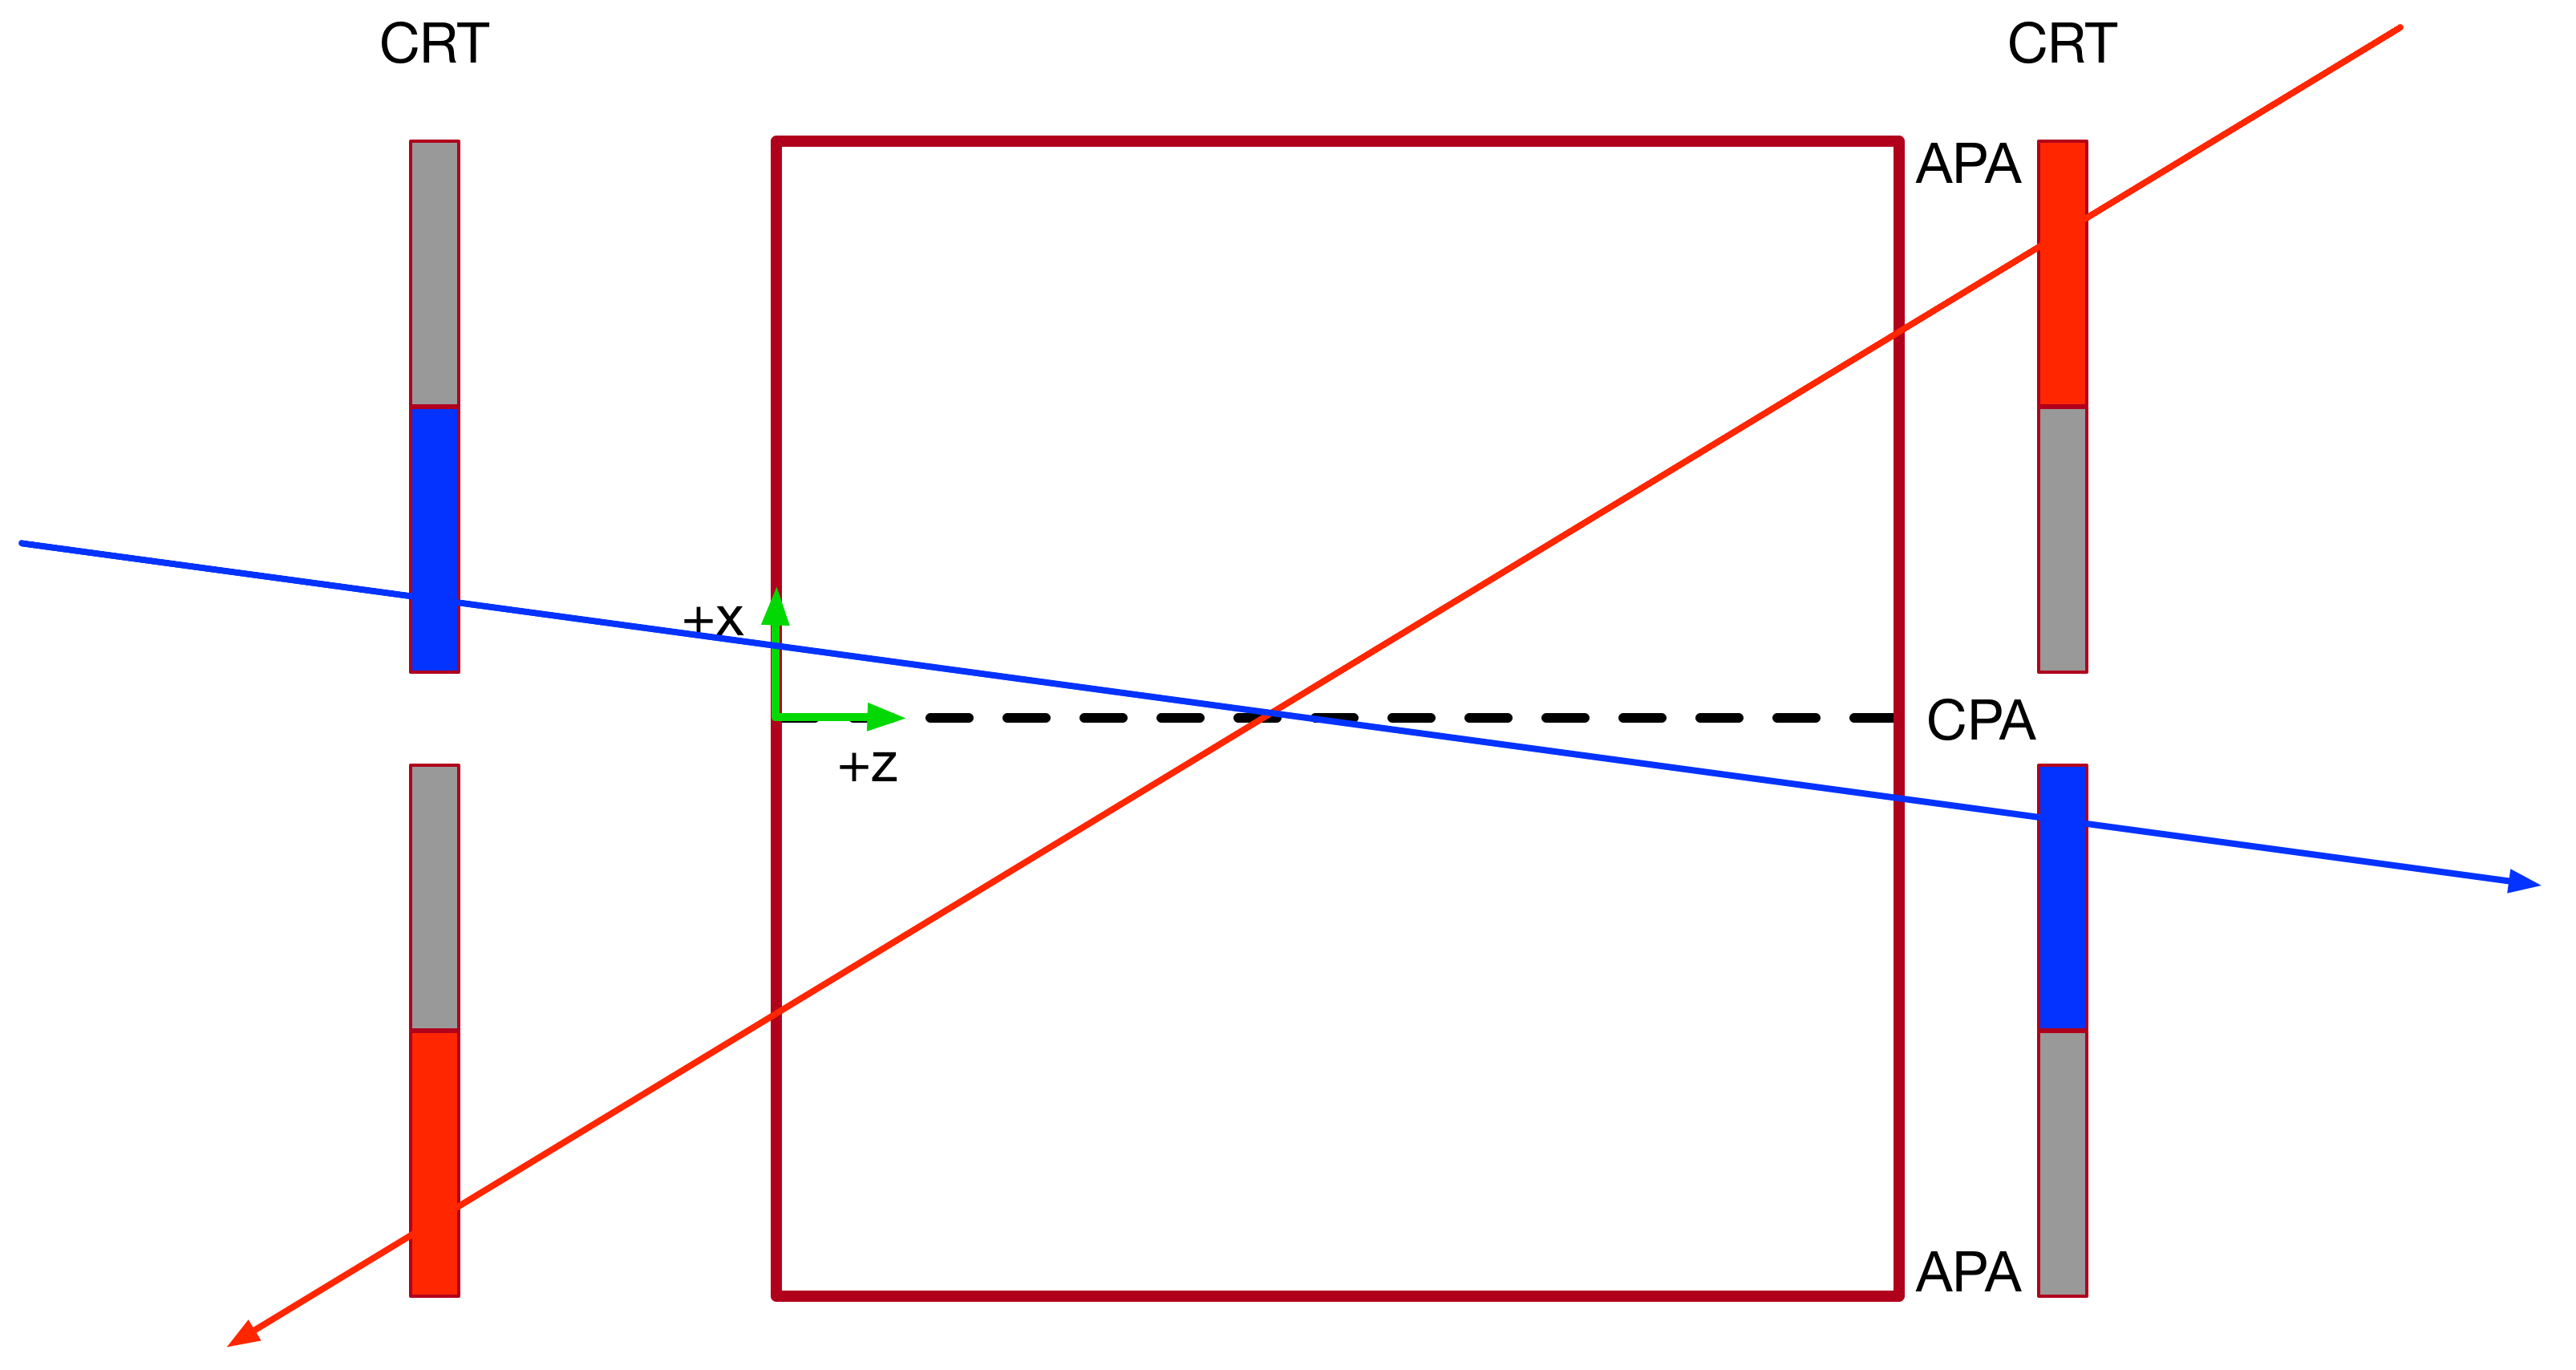
\includegraphics[width=9cm,height=4.5cm]{figs/pd_cosmic_top.png}
		\end{figure}
		
		\begin{itemize}
			\item Top to bottom cosmic tracks
			\item How precise (relatively) do we want to get with this, for a first go?
			\item Something like (1 OR 2) AND (25 OR 26)
		\end{itemize}
}

	\frame {
		\frametitle{CRT Trigger  1/}
		\framesubtitle{CRT Triggers Side View}
		\begin{figure}
			\centering
			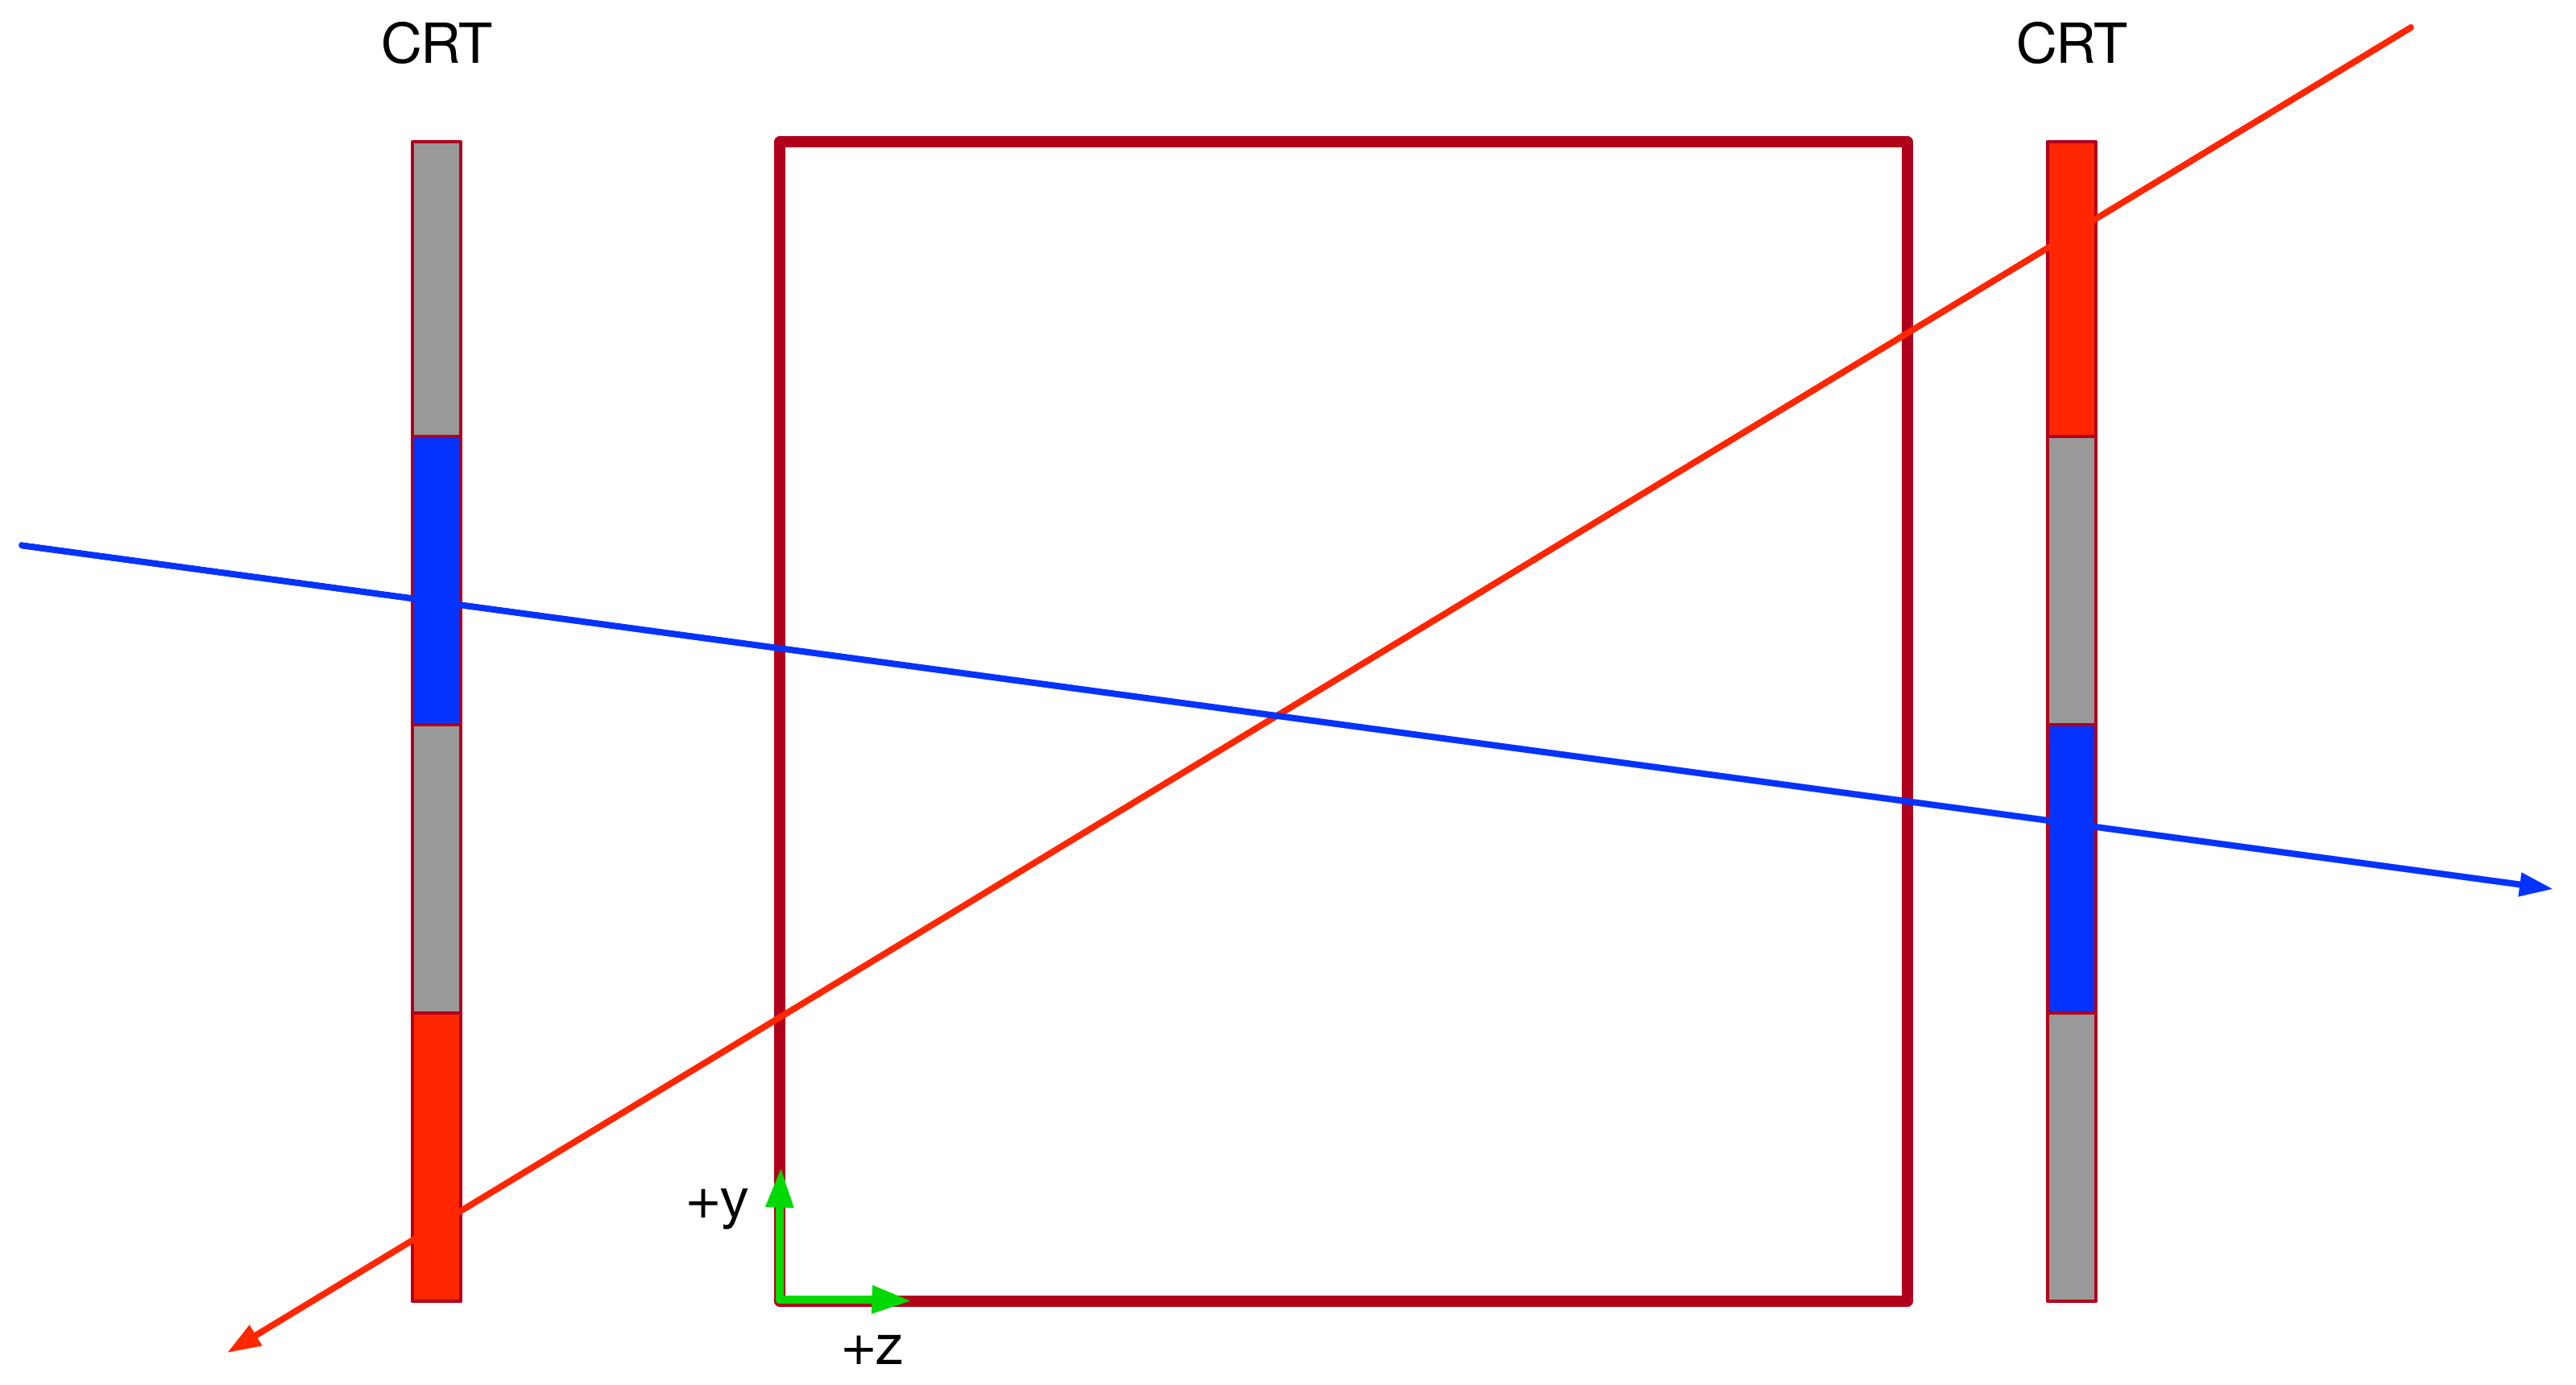
\includegraphics[width=9cm,height=4.5cm]{figs/pd_cosmic_side.png}
		\end{figure}
		
		\begin{itemize}
			\item Top to bottom cosmic tracks
			\item How precise (relatively) do we want to get with this, for a first go?
			\item Something like (1 OR 2) AND (23 OR 24)
		\end{itemize}
	}
	
	\frame {
		\frametitle{CRT Trigger Summary 1/}
		\framesubtitle{Channel Mapping of CRT Modules  (ref. Camillo M.)}
		
		\begin{itemize}
			\item Top to bottom cosmic tracks
			\item How precise (relatively) do we want to get with this, for a first go?
			\item Something like (1 OR 2) AND (25 OR 26)
		\end{itemize}
		
	\begin{center}
		\begin{table}[ht]	
			\caption{1-2 GeV/c beam triggers inclusive trigger masks.}
			\centering 
			\begin{tabular}{c c }
				\hline \hline         
				Trigger & CRT Channels $\lbrack$ 31 : 0 $\rbrack$ =[Rear, Front]  \\ [0.5ex] 
				\hline 
				No Beam & 0 XX X XXXXX  \\	
				e$^-$ & 1 11 1 11111  \\
				$\pi$/K/p & 1 00 1 11111  \\
				\hline	
			\end{tabular}
			\label{table:crt_trig}	
		\end{table}	
	\end{center}		
	}
	
	\frame {
		\frametitle{PDS Trigger  1/}
		\framesubtitle{}
		
		\begin{itemize}
			\item Don't have any of the PDS channel mappings
			\item On the SSPs some threshold set to discriminate on the SiPM signal sums.
			\item Counting trigger on PDS channels spatially near each other in the detector.
			\begin{itemize}
				\item E.g., only look at photon detectors in the TPCs on the side of the beam (+x side) during beam and require greater than some number to send a signal.
			\end{itemize}
			\item Inclusive trigger on the result of the counting triggers. 
		\end{itemize}
	}
	
	
\end{document}